\documentclass[12pt, a4paper]{report}
\usepackage{style}


\title{Image Analysis And Computer Vision \\ \textit{Theory}}
\author{Christian Rossi}
\date{Academic Year 2023-2024}

\begin{document}

\maketitle

\newpage

\begin{abstract}
    The topics of the course are: 
    \begin{itemize}
        \item Introduction.
        \item Camera sensors: transduction, optics, geometry, distortion
        \item Basics on Projective geometry: modelling basic primitives (points, lines, planes, conic sections, quadric surfaces) and projective spatial transformations and  projections.
        \item Camera geometry, and single view analysis: calibration, image rectification, localization of 3D models.
        \item Multi-view analysis: 3D shape reconstruction, self-calibration, 3D scene understanding.
        \item Linear filters and convolutions, space-invariant filters, Fourier Transform, sampling and aliasing. 
        \item Nonlinear filters: image morphology and morphology operators (dilate, erode, open, close), median filters.
        \item Edge detection and feature detection techniques. Feature matching and feature tracking along image sequences.
        \item Inferring parametric models from noisy data (including outliers), contour segmentation, clustering, Hough Transform, Ransac (random sample consensus). 
        \item Applications: object tracking, object recognition, classification.
    \end{itemize}
\end{abstract}

\cleardoublepage
\pagenumbering{Roman}

\tableofcontents

\cleardoublepage
\pagenumbering{arabic}

\chapter{Optical sensors}
    \section{Camera}
    \begin{definition}
    The \emph{camera} functions as an optical sensor, generating data through electric transducers. 
    It incorporates an optical system that directs incoming light at each of its millions of photosensitive elements. 
    Modern cameras typically have the capability to record 30 to 60 frames per second.
    \end{definition}
    For the sake of simplicity, we assume that the optical system of a camera consists of a single lens with the following characteristics:
    \begin{itemize}
        \item Spherical: the lens is created by the intersection of two spherical surfaces.
        \item Thin: the distance between the centers of the two spheres is nearly equal to the sum of their radius.
        \item Small angles: the light rays make only slight inclinations with respect to the optical axis.
    \end{itemize}
    These simplifications facilitate the calculation of the path of a ray as it passes through the lens.
    Specifically, the refraction of light when it crosses the boundary between two media is governed by Snell's law:
    \[\dfrac{\sin{\theta_2}}{\sin{\theta_1}}=\dfrac{n_1}{n_2}\]
    Here: 
    \begin{itemize}
        \item $\theta_1$ and $\theta_2$ represent the angles between the normal at the surface and the direction of the light ray before and after crossing the boundary, respectively.
        \item $n_1$ and $n_2$ are the refractive indices of the two materials.
    \end{itemize}
    \begin{figure}[H]
        \centering
        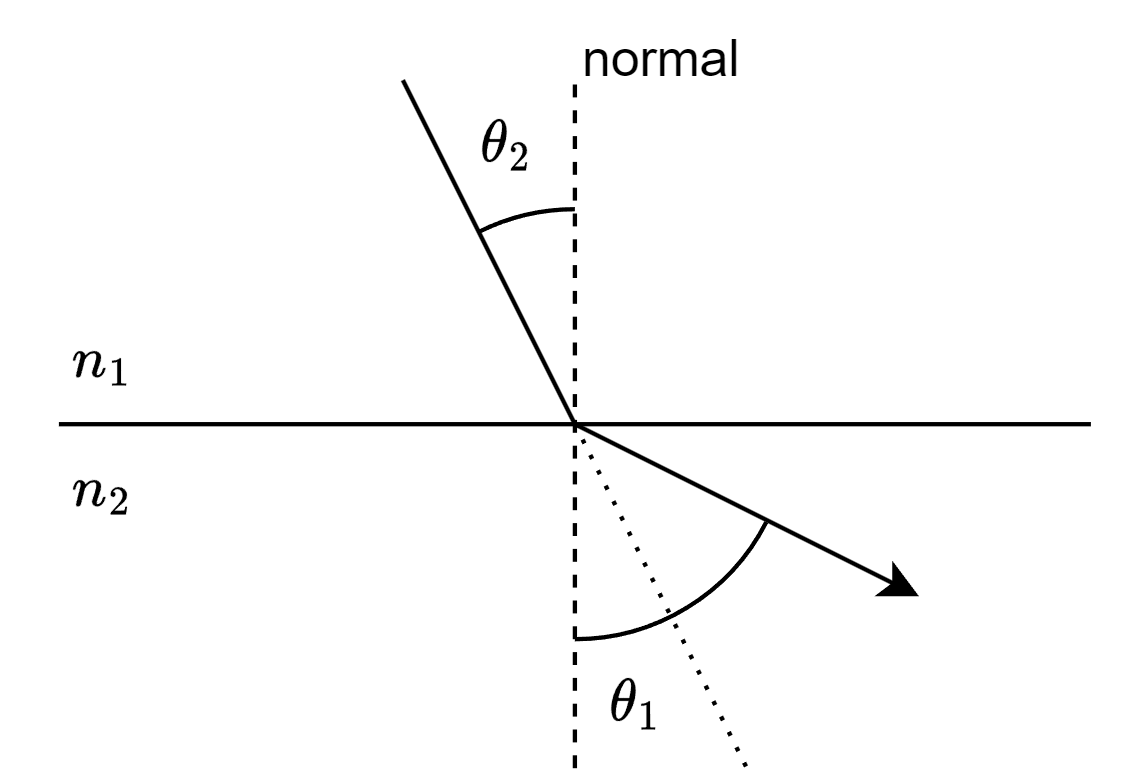
\includegraphics[width=0.4\linewidth]{images/refraction.png}
        \caption{Snell's law}
    \end{figure}
    \begin{definition}
        The \emph{optical axis} is the straight line that connects the center of the two spheres that compose the lens.
    \end{definition}
    The angles of a ray passing through the centers of the spheres can be determined as follows:
    \[\alpha_1=\dfrac{y_1}{\rho_1} \:\:\:\:\:\: \alpha_2=-\dfrac{y_2}{\rho_2}\]
    \begin{figure}[H]
        \centering
        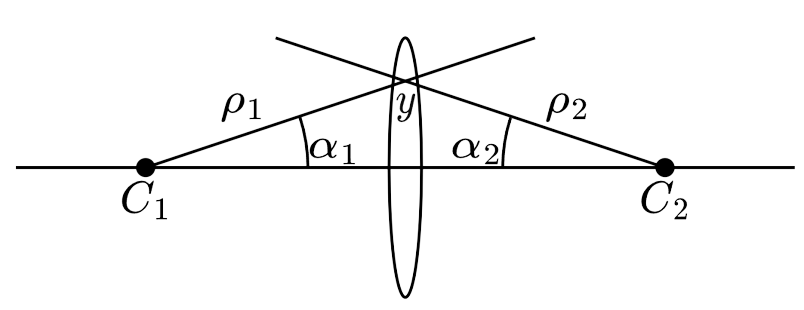
\includegraphics[width=0.4\linewidth]{images/y.png}
    \end{figure}
    In this context, with a simplified lens, it's valid to assume:
    \[y_1=y_2=y\]
    
    \section{Light rays deviation}
    \begin{figure}[H]
        \centering
        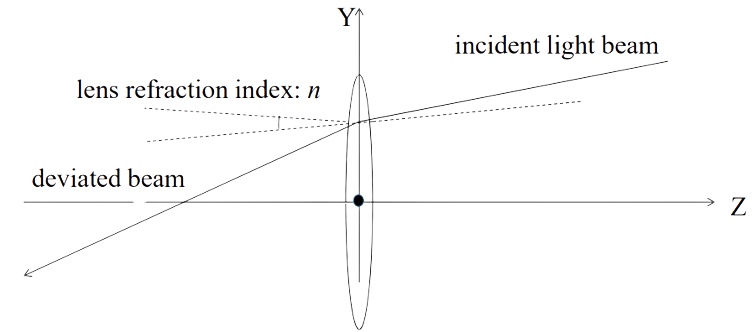
\includegraphics[width=0.4\linewidth]{images/ray.png}
    \end{figure}
    For a lens with a refractive index of $n$, the following equations hold true:
    \[\dfrac{\theta-\alpha_1}{\theta^{'}-\alpha_1} \Rightarrow \dfrac{\sin{(\theta-\alpha_1)}}{\sin{(\theta^{'}-\alpha_1)}}=n\]
    \[\dfrac{\theta^{''}-\alpha_2}{\theta^{'}-\alpha_2} \Rightarrow \dfrac{\sin{(\theta^{''}-\alpha_2)}}{\sin{(\theta^{'}-\alpha_2)}}=n\]
    Where:
    \begin{itemize}
        \item $\theta$ is the angle before the lens. 
        \item $\theta^{'}$ is the angle within the lens (not visible in the image). 
        \item $\theta^{''}$ is the angle after the lens.
    \end{itemize}
    By comparing these two equations, it is possible to determine the difference between the input angle $\theta$ and the output angle $\theta^{''}$, which can be expressed as:
    \[\delta \theta=y(n-1)\left( \dfrac{1}{\rho_1} + \dfrac{1}{\rho_2}\right)\]
    It is evident that the first term $(n-1)$is a result of the lens material, while the second term $\left( \frac{1}{\rho_1} + \frac{1}{\rho_2}\right)$ depends on the curvature of the lens surfaces.

    \section{Focalization of parallel light rays}
    \begin{figure}[H]
        \centering
        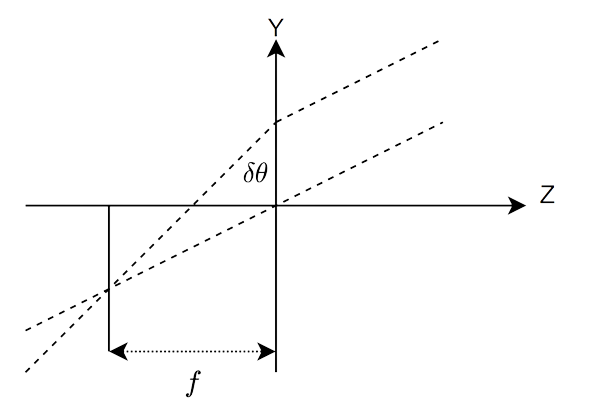
\includegraphics[width=0.4\linewidth]{images/focalization.png}
    \end{figure}
    In the image, we observe two rays: one passing through the center of the lens and another passing through a different point but remaining parallel to the first ray. 
    Consequently, we can make the following observations:
    \begin{itemize}
        \item When $Y = 0$, the ray experiences no deviation and continues without being deflected.
        \item Using the relationship $Y=f\cdot\delta\theta$, we can determine the focal length of the lens as follows: $f=\dfrac{1}{(n-1)\left(\dfrac{1}{\rho_1}+\dfrac{1}{\rho_2}\right)}$. 
    \end{itemize}
    This implies that all parallel rays converge to a common point, the focal point denoted as $Z$. 
    The distance of this focal point from the $Y$ axis is given by:
    \[Z=-f\]

    \section{Path of a light ray}
    To determine the projection of a light ray as it passes through a lens at any given position, the following steps can be followed:
    \begin{enumerate}
        \item Draw a line parallel to the chosen ray, passing through the center of the lens. 
        \item Identify the intersection point of this line with the focal plane.
        \item The ray will travel from the point where it crosses the lens to the point located on the focal plane.
    \end{enumerate}
    \begin{figure}[H]
        \centering
        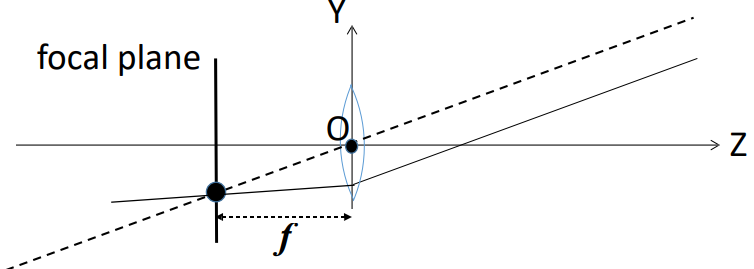
\includegraphics[width=0.4\linewidth]{images/path.png}
        \caption{Path of a light ray through a lens}
    \end{figure}

    \section{Pin-hole camera}
    To achieve a sharply focused image, it is essential that each light ray converges precisely onto a single pixel on the camera's focal plane. 
    To ensure this, we must satisfy the following conditions:
    \begin{itemize}
        \item The distance between the lens and the source of the ray, denoted as $Z(P)$, should be significantly greater than the lens aperture $a$, preferably at least a factor of 1000 times.
        \item By positioning the screen at a distance $Z$ from the lens, we enable all the rays to maintain parallel trajectories as they pass through the lens, resulting in a well-focused image.
    \end{itemize}
    The camera described so far is commonly known as a pin-hole camera, and it requires the following characteristics:
    \begin{enumerate}
        \item A thin spherical lens.
        \item Utilization of small angles.
        \item Ensuring that $Z(P) \gg a$.
        \item Maintaining $Z=f$, where $f$ represents the focal length.
    \end{enumerate}

    \section{From real world to 2D images}
    Images exist on a 2D plane, whereas the real world is three-dimensional, resulting in a reduction of information compared to the original subject in the real world. 
    This reduction is due to the perspective projection, which has the following characteristics:
    \begin{itemize}
        \item Nonlinearity.
        \item Lack of shape preservation.
        \item Failure to maintain length ratios.
    \end{itemize}
    By applying the triangle equality, we can express this perspective projection as:
    \[x=f \dfrac{X}{Z} \:\:\:\:\:\: y=f \dfrac{Y}{Z}\]
    To mitigate information loss, one approach is to capture an image of a planar scene on a plane that is parallel to the image plane. 
    This necessitates that:
    \[Z=Z_0=\textnormal{constant}\]
    \begin{figure}[H]
        \centering
        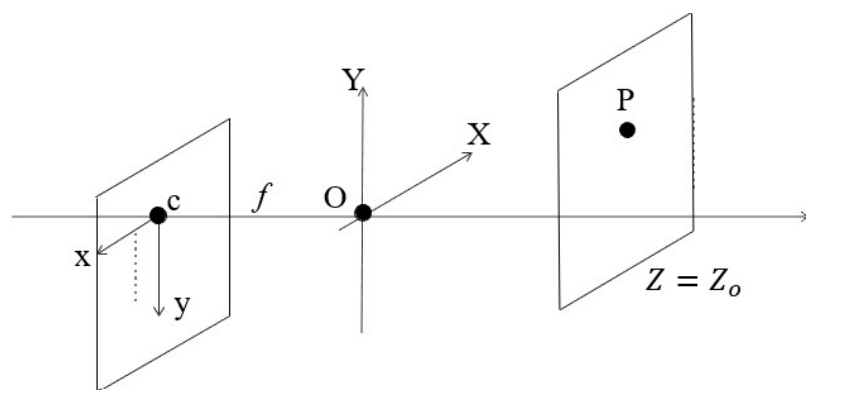
\includegraphics[width=0.5\linewidth]{images/Z0.png}
    \end{figure}
    In such a scenario, the sole distinction between reality and the projection is a uniform downscaling, while other dimensions are preserved, giving us:
    \[x=f \dfrac{X}{Z_0}=kX \:\:\:\:\:\: y=f \dfrac{Y}{Z_0}=kY \]
    
    \section{Perspective and vanishing point}
    If we opt to consider all lines parallel to the direction parameters $\begin{bmatrix} \alpha & \beta & 1 \end{bmatrix}$, we can establish the following system of equations:
    \[
        \begin{cases}
            X = X_0 + \alpha Z  \\
            Y = Y_0 + \beta Z   \\
            Z = 1 \cdot Z
        \end{cases}
    \]
    To project these lines onto the 2D image using the triangle equality, we derive the following expressions:
    \[x=f \dfrac{X}{Z} = f \dfrac{X_0 + \alpha Z}{Z} = f\alpha + \dfrac{X_0}{Z}\]
    \[y=f \dfrac{Y}{Z} = f \dfrac{Y_0 + \beta Z}{Z}  = f\beta  + \dfrac{Y_0}{Z}\]
    Now, let's find the image of the point at infinity along these lines, which yields the point:
    \[\begin{bmatrix} f\alpha & f\beta \end{bmatrix}\]
    Remarkably, this image point is independent of the values of $X_0$ and $Y_0$. 
    Hence, all parallel lines share the same image of their points at infinity.
    \newpage
    \begin{definition}
        The image of the point at the infinity of the lines is known as the \emph{vanishing point}. 
    \end{definition}
    As a result, we observe that all lines parallel in the real world project onto converging lines in the image.
    \begin{figure}[H]
        \centering
        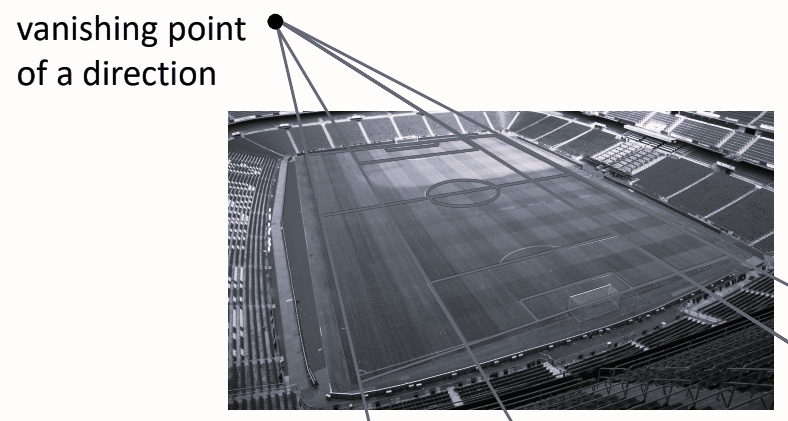
\includegraphics[width=0.4\linewidth]{images/vanishingpoint.png}
        \caption{Example of vanishing point}
    \end{figure}
    
\newpage

\chapter{Two-dimensional planar projective geometry}
    \section{Introduction}
    In the realm of planar geometry, the fundamental elements include points, lines, conics, and dual conics. 
    The permissible transformations within this geometry encompass projectivities, affinities, similarities, and isometries.

    \section{Points}
    To define points in Cartesian coordinates, a Euclidean plane is established, with a designated origin. 
    Each point is uniquely represented by a pair of Cartesian coordinates, $(x, y)$.

    For the analysis of images, it is advantageous to use homogeneous coordinates.
    To define this coordinate system, we construct a 3D space with axes labeled $x$, $y$, and $w$. 
    Now, to represent a point, we assign three values. 
    This implies that every point can have an infinite number of representations by altering the value of $w$.

    To analyze images it is better to use homogeneous coordinates. To define this type of coordinates we need to construct a 3D space with $x,y,w$ axis. So, now to define a point
    we have to assign three values. This means that every number can be represented in infinite ways by changing the value of $w$. 
    The relationship between Cartesian and homogeneous coordinates can be expressed as follows:

    \[
    x=
    \begin{bmatrix}
        x \\
        y \\
        w 
    \end{bmatrix}
    =w
    \begin{bmatrix}
        X \\
        Y \\
        1 
    \end{bmatrix}
    \]

    Consequently, a vector $x = {\begin{bmatrix} x & y & w \end{bmatrix}}^T$ and all its nonzero multiples, including ${\begin{bmatrix} \frac{x}{w} & \frac{y}{w} & 1 \end{bmatrix}}^T$, represent the same point in Cartesian coordinates ${\begin{bmatrix} X & Y \end{bmatrix}}^T={\begin{bmatrix}  \frac{x}{w} &  \frac{y}{w} \end{bmatrix}}^T$ on the Euclidean plane. 
    This representation adheres to the homogeneity property: any vector $x$ is equivalent to all its nonzero multiples $\lambda x$, where $\lambda \neq 0$, since they denote the same point.
    The null vector does not represent any point.
    \newpage
    \begin{definition}
        Let's define the \emph{projective plane} as:
        \[\mathbb{P}^2=\{{\begin{bmatrix} x & y & w \end{bmatrix}}^T \in \mathbb{R}^3\}-\{{\begin{bmatrix} 0 & 0 & 0 \end{bmatrix}}^T\}\]
    \end{definition}
    \begin{example}
        The origin of the plane is defined as:
        \[{\begin{bmatrix} 0 & 0 & 1 \end{bmatrix}}^T\]
        A generic point in homogeneous coordinates can be easily transformed into a pair of Cartesian coordinates by a straightforward division. 
        For example, the point:
        \[{\begin{bmatrix} 0 & 8 & 4 \end{bmatrix}}^T\]
        in Cartesian coordinates is equal to:
        \[{\begin{bmatrix} \frac{x}{w} & \frac{y}{w} \end{bmatrix}}^T=\begin{bmatrix} \frac{0}{4} & \frac{8}{4} \end{bmatrix}=\begin{bmatrix} 0 & 4 \end{bmatrix}\]
    \end{example}
    Consider a point $x={\begin{bmatrix} x & y & w \end{bmatrix}}^T$, and let $w$ slowly decrease from $w=1$. 
    As $w$ decreases, moves along a constant direction $\begin{bmatrix} x & y \end{bmatrix}$, while distancing itself from the origin. 
    As $w$ approaches $0$, tends towards infinity along the direction $\begin{bmatrix} x & y \end{bmatrix}$. 
    \begin{definition}
        We define the \emph{point at the infinity along the direction} $\begin{bmatrix} x & y \end{bmatrix}$ as: 
        \[x=\begin{bmatrix} x \\ y \\ w \end{bmatrix}\]
    \end{definition}
    Points at the infinity, representing directions, exist outside the Euclidean plane, and they are additional points well-defined within the projective plane. 
    Therefore, the projective plane encompasses not only the Euclidean plane but also these points at infinity.

    \section{Lines}
    In the Euclidean plane, a line is typically defined by the equation:
    \[aX+bY+c=0\]
    However, in the homogeneous plane, lines are represented as:
    \[a\dfrac{x}{w}+b \dfrac{y}{w}+c=0 \Longrightarrow ax+by+cw=0\]
    This equation can also be expressed using two vectors, denoted as $l^T$ and $x$, as follows:
    \[\begin{bmatrix} a & b & c \end{bmatrix} \begin{bmatrix} x \\ y \\ w \end{bmatrix}=0\]
    Here, the vector $l={\begin{bmatrix} a & b & c \end{bmatrix}}^T$, and all its nonzero multiples represent a line.  
    This representation adheres to the homogeneity property: any vector $l$ is equivalent to all its nonzero multiples, denoted as $\lambda l$, where $\lambda\neq 0$, since they denote the same line. 
    The coefficients $a$, $b$, and $c$ are referred to as the homogeneous parameters of the line.
    
    Similar to numbers, there exist numerous equivalent representations for a single line, specifically all nonzero multiples of the unit normal vector. 
    The null vector, however, does not represent any lines.
    \begin{definition}
        The \emph{projective dual plane} is defined as: 
        \[\mathbb{P}^2=\{{\begin{bmatrix} a & b & c \end{bmatrix}}^T \in \mathbb{R}^3\}-\{{\begin{bmatrix} 0 & 0 & 0 \end{bmatrix}}^T\}\]
    \end{definition}

    \begin{property}
        If the third parameter is zero, denoted as ${l=\begin{bmatrix} a & b & 0 \end{bmatrix}}^T$, then the line passes through the point $\begin{bmatrix} 0 & 0 \end{bmatrix}$. 
    \end{property}
    \begin{property}
        In the Euclidean plane, the direction $\begin{bmatrix} a & b \end{bmatrix}$ is perpendicular to the line represented by ${l=\begin{bmatrix} a & b & c \end{bmatrix}}^T$.
    \end{property}
    \begin{property}
        Two lines, ${l=\begin{bmatrix} a & b & c \end{bmatrix}}^T$ and ${l=\begin{bmatrix} a & b & c^{'} \end{bmatrix}}^T$, are considered parallel when they share the same direction, which is represented by $[b,-a]$.
    \end{property}
    \begin{example}
        The Cartesian axes are defined as: 
        \[l_x={\begin{bmatrix} 0 & 1 & 0 \end{bmatrix}}^T\]
        \[l_y={\begin{bmatrix} 1 & 0 & 0 \end{bmatrix}}^T\]
    \end{example}
    In this context, the incidence relation of a line $l^Tx=0$ is defined when the point $x$ lies on the line $l$ or when the line $l$ goes through the point $x$. 
    \begin{definition}
        The line 
        \[\begin{bmatrix} 0 & 0 & 1 \end{bmatrix} \begin{bmatrix} x \\ y \\ w \end{bmatrix}=w=0\] 
        is called the \emph{line at the infinity}, denoted as $l_{\infty}={\begin{bmatrix} 0 & 0 & 1 \end{bmatrix}}^T$. 
    \end{definition}
    The principle of duality between points and lines states that the incidence relation is commutative since the dot product is commutative.

    To find the intersection of two lines $l_1$ and $l_2$, the following condition is imposed:
    \[\begin{bmatrix} l_1^T \\ l_2^T \end{bmatrix} x = \begin{bmatrix} 0 \\ 0 \end{bmatrix}\]
    This equation leads to finding the right null space of the first column vector:
    \[x=\textnormal{RNS}\left(\begin{bmatrix}l_1^T \\ l_2^T \end{bmatrix} \right)\]
    The system is under-determined, meaning there is only one intersection point between two lines, which can be represented in multiple ways in homogeneous coordinates.
    In 2D projective geometry, the vector $x$ is orthogonal to both lines and can be found using the cross product:
    \[x=l_1 \times l_2\]
    \begin{example}
        Suppose we have two parallel lines, $l_1={\begin{bmatrix} a & b & c_1 \end{bmatrix}}^T$ and $l_2={\begin{bmatrix} a & b & c_2 \end{bmatrix}}^T$. 
        The point that is common to both lines can be found using the system:
        \[
            \begin{cases}
                ax+by+c_1w=0 \\
                ax+by+c_2w=0
            \end{cases}
        \]
        The solution is ${x=\begin{bmatrix} b & -a & 0 \end{bmatrix}}^T$, which represents the point at infinity along the direction of both lines.
    \end{example}

    The line passing through two points can be determined using the dual of the previous problem, expressed as:
    \[\begin{bmatrix} x_1^T \\ x_2^T \end{bmatrix} l = \begin{bmatrix} 0 \\ 0 \end{bmatrix}\]
    In 2D, this simplifies to: 
    \[l=x_1 \times x_2\] 
    \begin{property}
        A point $x$ obtained by a linear combination $x=\alpha x_1+\beta x_2$ of two points $x_1$ and $x_2$ lies on the line $l$ through $x_1$ and $x_2$. 
    \end{property}
    \begin{proof}
        The line $l$ passing through both points satisfies  $l^Tx_1=0$ and  $l^Tx_2=0$. 
        By adding $\alpha$ times the first equation to $\beta$ times the second one, we obtain: 
        \[0=l^T\left( \alpha x_1+\beta x_2 \right)=l^Tx=0\]
    \end{proof}
    This establishes the duality between co-linear and concurrent.
    \begin{theorem}
        For any true sentence containing the words: point, line, is on, goes through, co-linear and concurrent there exists a dual sentence (also true) obtained by replacing each occurrence of:
        \begin{itemize}
            \item Point $\Leftrightarrow$ line. 
            \item Is on $\Leftrightarrow$ goes through.
            \item Co-linear $\Leftrightarrow$ concurrent. 
        \end{itemize}
    \end{theorem}
    Within the euclidean plane, the direction normal to the line $l={\begin{bmatrix} a & b & c \end{bmatrix}}^T$ is represented by $\begin{bmatrix} a & b \end{bmatrix}$. 
    This relationship between lines can be explained by understanding that the angle between two lines is equal to the angle between their respective normal vectors. 
    The formula for the angle between two vectors is:
    \[\cos\theta=\dfrac{u \cdot v}{\left\lvert u \right\rvert \left\lvert v \right\rvert}\] 
    This applies to the angle between two lines $l_1={\begin{bmatrix} a_1 & b_1 & c_1 \end{bmatrix}}^T$ and $l_2={\begin{bmatrix} a_2 & b_2 & c_2 \end{bmatrix}}^T$. 
    In this context, it is the angle between their respective normal directions $\begin{bmatrix} a_1 & b_1 \end{bmatrix}$ and $\begin{bmatrix} a_2 & b_2 \end{bmatrix}$, which can be calculated as follows:
    \[\cos\theta=\dfrac{a_1a_2+b_1b_2}{\sqrt{\left( a_1^2 + b_1^2 \right)\left( a_2^2 + b_2^2 \right)}}\]
    
    Now, consider a line with four points related as follows:
    \[X_1=\alpha_1Y+\beta_1Z\]
    \[X_2=\alpha_2Y+\beta_2Z\]
    The cross ratio is given by:
    \[CR_{X_1,X_2,Y,Z}=\dfrac{c-a}{c-b}/\dfrac{d-a}{d-b}=\dfrac{\beta_1/\alpha_1}{\beta_2/\alpha_2}\]
    \begin{figure}[H]
        \centering
        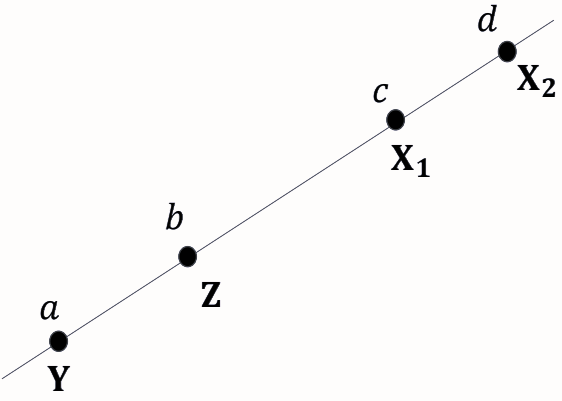
\includegraphics[width=0.25\linewidth]{images/line.png}
        \caption{Line with the point of previous problem}
    \end{figure}
    \begin{proof}
        Since the abscissae are proportional, the abscissae can be replaced by the $X$ coordinate, as illustrated in the figure below:
        \begin{figure}[H]
            \centering
            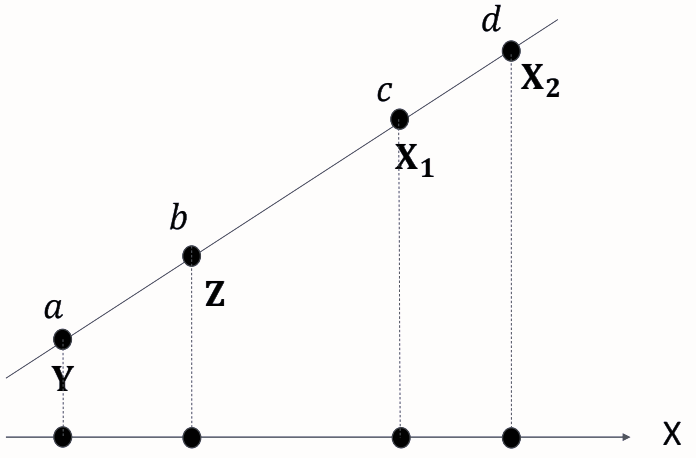
\includegraphics[width=0.3\linewidth]{images/abscissae.png}
        \end{figure}
        The relation:
        \[CR_{X_1,X_2,Y,Z}=\dfrac{c-a}{c-b}/\dfrac{d-a}{d-b}\]
        still holds. 
        If we consider $Y={\begin{bmatrix} y & * & v \end{bmatrix}}^T$ and $Z={\begin{bmatrix} z & * & w \end{bmatrix}}^T$, we can determine that:
        \[ X_1=\begin{bmatrix} \alpha_1y+\beta_1z \\ * \\ \alpha_1v+\beta_1w \end{bmatrix} \:\:\:\:\:\:\:\:\:\:\:\: X_2=\begin{bmatrix} \alpha_2y+\beta_2z \\ * \\ \alpha_2v+\beta_2w \end{bmatrix}\]
        The difference between the $X$ coordinates of $X_1$ and $Y$ is calculated as:
        \[c-a=\dfrac{\beta_1(zv-yw)}{(\alpha_1y+\beta_1z)v}\]
        Similarly, the difference between the $X$ coordinates of $X_1$ and $Z$ is:
        \[c-b=\dfrac{-\alpha_1(zv-yw)}{(\alpha_1y+\beta_1z)w}\]
        By substituting these expressions, we obtain:
        \[ \dfrac{c-a}{c-b}=-\dfrac{\beta_1w}{\alpha_1v} \:\:\:\:\:\:\:\:\:\:\:\: \dfrac{d-a}{d-b}=-\dfrac{\beta_2w}{\alpha_2v}\]
    \end{proof}

    \section{Conics}
    Conics are geometric shapes that result from the intersection of cones with planes. 
    They include circles, ellipses, parabolas, and hyperbolas, as depicted in the following figure:
    \begin{figure}[H]
        \centering
        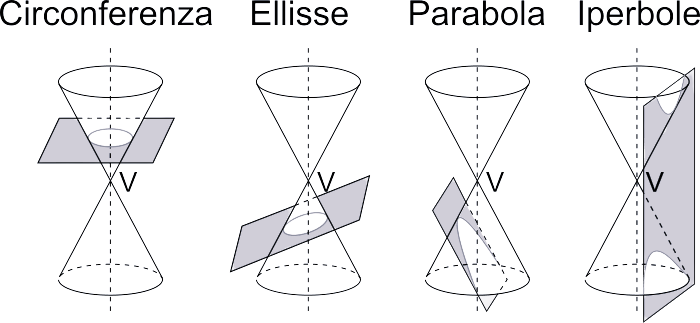
\includegraphics[width=0.5\linewidth]{images/conics.png}
    \end{figure}
    \begin{definition}
        A point $x$ is considered to be on a \emph{conic} $C$ if it satisfies a homogeneous quadratic equation of the form:
        \[x^TCx=0\]
        Where $C$ is a symmetric matrix is a symmetric matrix, which is a convention.
    \end{definition}
    Conics are curves described by second-degree equations in the plane. 
    In Euclidean coordinates, a conic can be expressed as:
    \[aX^2+bXY+cY^2+dX+eY+f=0\]
    In homogeneous coordinates, it becomes:
    \[ax^2+bxy+cy^2+dxw+eyw+fw^2=0\]
    Alternatively, it can be represented in matrix form as:
    \[x^T \begin{bmatrix} a & b/2 & d/2 \\ b/2 & c & e/2 \\ d/2 & e/2 & f \end{bmatrix} x=0\]
    Conics have five degrees of freedom, which means that five points are required to uniquely define a conic.
    \begin{example}
        A circle can be expressed in Cartesian coordinates as:
        \[(X-X_0)^2+(Y-Y_0)^2-r^2=0\]
        In homogeneous coordinates, it is represented as:
        \[  \begin{bmatrix} x & y & w \end{bmatrix}
            \begin{bmatrix} 1 & 0 & -X_0 \\ 0 & 1 & -Y_0 \\ -X_0 & -Y_0 & X_0^2+Y_0^2-r^2 \end{bmatrix}
            \begin{bmatrix} x \\ y \\ w \end{bmatrix} = 0
        \]
    \end{example}

    When you have a quadratic equation representing a conic and a linear equation for a line, their intersection results in a second-degree equation for the point $x$. 
    Consequently, there will always be two intersection points between a line and a conic. 
    These intersection points can fall into one of the following categories:
    \begin{itemize}
        \item Real and distinct: this occurs when the line and conic intersect at two separate, real points.
        \item Real and coincident: in this case, the line and conic intersect at a single real point, but it is a repeated or double root of the equation.
        \item Complex and distinct: the intersection points are two complex conjugate points.
        \item Complex and coincident: the line and conic intersect at a single complex point, and it is a repeated or double root.
    \end{itemize}
    This behavior is due to the fundamental theorem of algebra, which guarantees that a second-degree equation will have exactly two solutions when considering complex numbers.
    \begin{figure}[H]
        \centering
        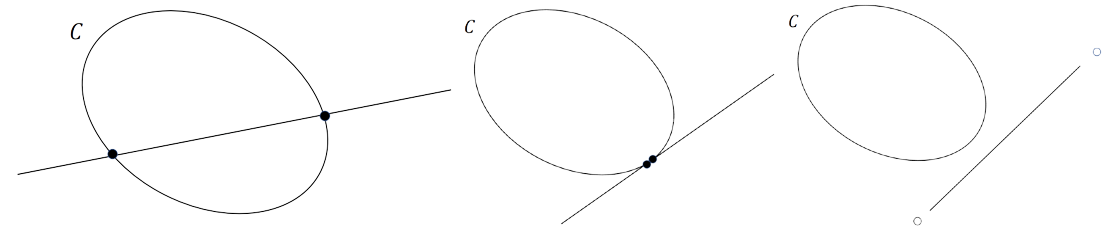
\includegraphics[width=0.75\linewidth]{images/intersection.png}
        \caption{Intersection with two real roots, two coincident roots and two imaginary roots}
    \end{figure}
    The intersection between the line at infinity and a conic results in the following scenarios:
    \begin{itemize}
        \item Parabola: when there are two coincident solutions, indicating the point at infinity along the axis.
        \item Ellipse: when there are two complex-conjugate solutions, meaning there are no real solutions.
        \item Hyperbola: when there are two real and distinct solutions, representing lines that serve as the asymptotes.
    \end{itemize}

    \subsection{Circular points}
    \begin{example}
        When we intersect a circumference and the line at infinity, we obtain the following system:
        \[\begin{cases}
            x^2-2X_0w+X_0^2w^2+y^2-2Y_0w+Y_0^2w^2-r^2w^2=0 \\
            w=0
        \end{cases}\]
        This system simplifies to: 
        \[x^2+y^2=0\]
        It's evident that the parameters of the circumference (center and radius) have disappeared from the equation. 
        Consequently, the two intersection points are the same for all circumferences.    
    \end{example}
    \newpage
    \begin{definition}
        The two intersection points remain the same for all circumferences when intersected with the line at infinity are referred to as the \emph{circular points}.
        These points are defined as:
        \[I=\begin{bmatrix} 1 \\ i \\ 0 \end{bmatrix} \:\:\:\:\:\: J=\begin{bmatrix} 1 \\ -i \\ 0 \end{bmatrix}\]
    \end{definition}

    \subsection{Polar line}
    \begin{definition}
        Given a point $y$ and a conic $C$ in the plane, the line $l=Cy$ is called the \emph{polar line} of point $y$ with respect to the conic $C$. 
    \end{definition}
    \begin{figure}[H]
        \centering
        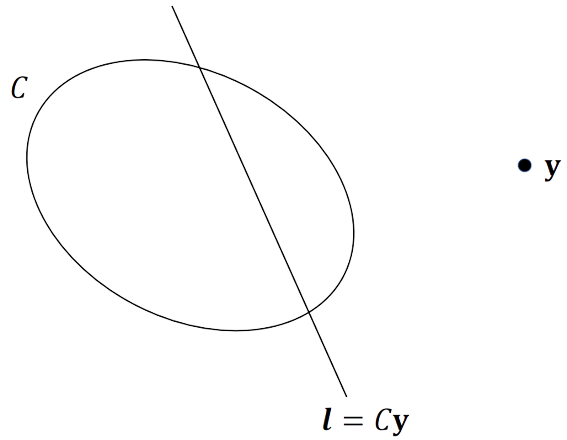
\includegraphics[width=0.3\linewidth]{images/polar.png}
        \caption{Example of polar line}
    \end{figure}
    
    \subsection{Harmonic tuples}
    \begin{definition}
        A 4-tuple of co-linear points A, B, C, D, whose cross ratio is = -1, is referred to as a \emph{harmonic tuple}. 
    \end{definition}
    This specific value of the cross ratio is also shared by other 4-tuples of co-linear points. 
    A notable example is:
    \[\left( T,Z,\textnormal{mid\_point}(Y,Z),P(\textnormal{at the infinity}) \right)\]
    Furthermore, if $(A, B, C, D)$ is a harmonic 4-tuple, then $(C, D, A, B)$ is also harmonic. 
    \begin{definition}
        In a harmonic tuple $(A, B, C, D)$, points $A$ and $B$ are said to be \emph{conjugate} of each other concerning points $C$ and $D$.
    \end{definition}
    Since the cross ratio of a harmonic tuple is negative, it follows that two conjugate points, $A$ and $B$, concerning $C$ and $D$, are positioned in such a way that one is located within the segment ($C, D$), while the other is situated outside this segment.

    \subsection{Polar line and harmonic tuples}
    Take any point $z$ on the polar line $l=Cy$ and then consider the line passing through points $y$ and $z$. 
    Let's denote by $x_1$ and $x_2$ the points at which this line intersects the conic.    
    \begin{figure}[H]
        \centering
        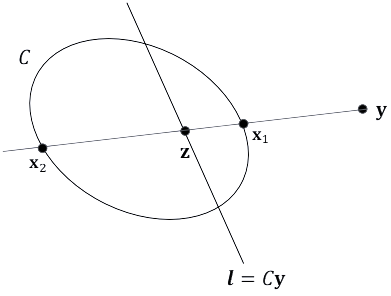
\includegraphics[width=0.25\linewidth]{images/polarharmonic.png}
    \end{figure}
    \begin{theorem}
        Let $x_1$ and $x_2$ represent the points at which the line passing through $y$ and $z$ intersects the conic $C$. 
        In this case, $y$ and $z$ are conjugate with respect to $x_1$ and $x_2$.     
    \end{theorem}
    The polar line $l=Cy$ represents the set of points that are conjugate to $y$ with respect to the conic $C$.
    More precisely, it includes points that are conjugate with respect to the intersection points of $C$ with any line passing through $y$.

    \subsection{Polar line and tangency points}
    As the line through $y$ approaches tangency with the conic $C$, the points $x_1$ and $x_2$ coincide with the points of tangency to $C$. 
    Consequently, the conjugate point $z$, which remains within the interval ($x_1,x_2$), also coincides with the tangency point. 
    This applies to any line that is tangent to $C$ from the point $y$.
    Therefore, we have established that the polar line $l=Cy$ passes through the points of tangency from $y$ to the conic $C$. 

    This leads us to the conclusion that if a point $z$ lies on the conic $C$, then point $y$ is one of its conjugates with respect to the same conic. 
    The tangent line $lz$ to the conic $C$ passing through point $z$ is the set of points that are conjugate to $z$. 
    Therefore, we can assert that $lz$ is the polar line of $z$ with respect to conic $C$.
    \begin{figure}[H]
        \centering
        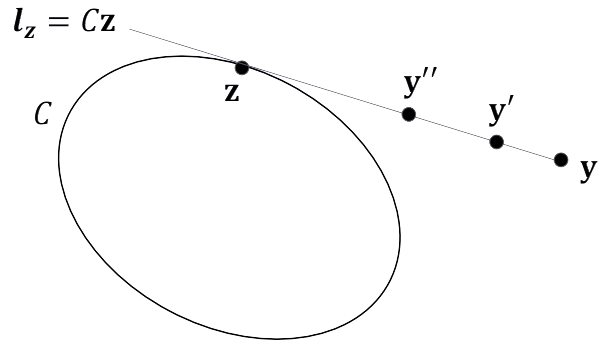
\includegraphics[width=0.4\linewidth]{images/tangentpolar.png}
    \end{figure}
    In the accompanying illustration, you can observe that the polar line $lz = Cz$ for a point $z$ situated on the conic $C$ corresponds to the tangent line to the conic $C$ at the point $z$.
    \begin{example}
        Consider a circumference with radius $r$ centered in the origin of the plane and the point $y={\begin{bmatrix} X & 0 & 1 \end{bmatrix}}^T$. 
        The equation of the polar line is given by:
        \[
        l=Cy=
        \begin{bmatrix}
            1 & 0 & 0 \\
            0 & 1 & 0 \\
            0 & 0 & -r^2
        \end{bmatrix}    
        \begin{bmatrix}
            X \\
            0 \\
            1 
        \end{bmatrix}    
        = 
        \begin{bmatrix}
            X \\
            0 \\
            -r^2 
        \end{bmatrix}  
        \]
        Therefore, the Cartesian equation of the polar line becomes: 
        \[X x-r^2 = 0 \rightarrow x=\dfrac{r^2}{X}\]
        This equation describes a vertical line.
    \end{example}

    From the previous example, we can conclude that the polar of a point $P$ with respect to a circle is a line that is perpendicular to the line segment connecting the center of the circle to point $P$. 
    \begin{example}
        Consider a circumference with radius $r$ centered in the origin of the plane and the point $y={\begin{bmatrix} x & 0 & 0 \end{bmatrix}}^T$.
        The equation of the polar line is given by:
        \[
        l=Cy=
        \begin{bmatrix}
            1 & 0 & 0 \\
            0 & 1 & 0 \\
            0 & 0 & -r^2
        \end{bmatrix}    
        \begin{bmatrix}
            x \\
            0 \\
            0 
        \end{bmatrix}    
        = 
        \begin{bmatrix}
            X \\
            0 \\
            0 
        \end{bmatrix}  
        \]
        Therefore, the Cartesian equation of the polar line becomes: 
        \[X x=0 \rightarrow X=0\]
        This equation describes the diameter of the circumference perpendicular at the direction of the point $y$. 
    \end{example}
    Tangent lines emerging from a point at infinity are always parallel. 
    Consequently, the points of tangency lie along a diameter that is perpendicular to the direction of these parallel tangents.    
    \begin{figure}[H]
        \centering
        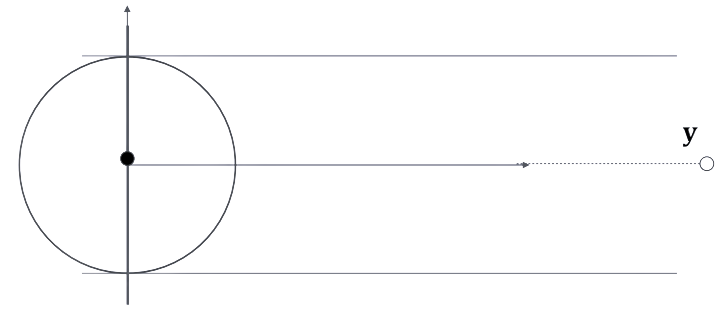
\includegraphics[width=0.5\linewidth]{images/parallel.png}
    \end{figure}
    \begin{example}
        Consider a circumference with radius $r$ centered in the origin of the plane and the point $y={\begin{bmatrix} x & 0 & 0 \end{bmatrix}}^T$.
        The equation of the polar line is given by:
        \[
        l=Cy=
        \begin{bmatrix}
            1 & 0 & 0 \\
            0 & 1 & 0 \\
            0 & 0 & -r^2
        \end{bmatrix}    
        \begin{bmatrix}
            0 \\
            0 \\
            1 
        \end{bmatrix}    
        = 
        \begin{bmatrix}
            0 \\
            0 \\
            -r^2 
        \end{bmatrix}  
        \]
        Therefore, the Cartesian equation of the polar line becomes: 
        \[-r^2w=0 \rightarrow X=0\]
        This equation describes the line at the infinity. 
    \end{example}
    Here are the general properties of the polar lines.
    \begin{property}
        The polar line of any point at infinity is a diameter.
    \end{property}
    \begin{property}
        Any diameter goes through the center of the circle.
    \end{property}
    \begin{property}
        The center is conjugate to every point at infinity.
    \end{property}
    \begin{property}
        All points at infinity are conjugate to the center.
    \end{property}
    \begin{property}
        The polar of the center is the line that includes all the points at infinity.
    \end{property}
    \begin{property}
        The polar line of the center is the line at infinity.
    \end{property}

    \subsection{Degenerate conics}
    \begin{definition}
        A \emph{non-degenerate conic} is a conic where the matrix $C$ is non-singular, indicating that: 
        \[\textnormal{rank}(C)=3\]

        Conversely, a \emph{degenerate conic} is a conic  for which the matrix $C$ is singular, characterized by: 
        \[\textnormal{rank}(C) < 3\]
    \end{definition}
    There are two distinct scenarios to consider:
    \begin{itemize}
        \item When $\textnormal{rank}(C) = 2$, any symmetric $3 \times 3$ matrix $C$ can be expressed as:
            \[C=lm^T+ml^T\]
            Here, $l$ and $m$ are column vectors. 
            The conic corresponds to the set of points $x$  that satisfy $x^TCx=0$.
            This equation is met when either $x^Tl=0$ or $m^Tx=0$. 
            Consequently, $x$ lies on the union of lines represented by $l$ and $m$
            \begin{figure}[H]
                \centering
                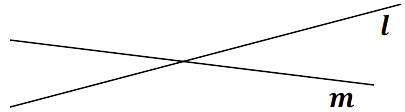
\includegraphics[width=0.25\linewidth]{images/inters.png}
            \end{figure}
        \item When $\textnormal{rank}(C) = 1$, a symmetric $3 \times 3$ matrix $C$ can be expressed as:
            \[C=ll^T\]
            In this case, $l$ is a column vector. 
            The conic consists of the points $x$ that satisfy $x^TCx=0$.
            This equation holds  when $x^Tl=0$ is met (twice). 
            Thus, $x$ is on the repeated line represented by $l$.
            \begin{figure}[H]
                \centering
                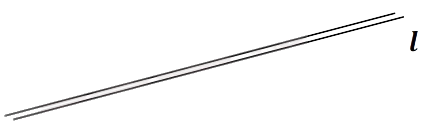
\includegraphics[width=0.25\linewidth]{images/rep.png}
            \end{figure}
    \end{itemize}

    \section{Dual conics}
    \subsection{Definition}
    \begin{definition}
        A \emph{dual conic} is a set of lines $l$ that satisfy equation:
        \[l^TC^{*}l=0\]
        where $C^{*}$ is a $3 \times 3$ symmetric matrix.

        A \emph{non-degenerate dual conic} is a dual conic whose matrix $C^{*}$ is non-singular: 
        \[\textnormal{rank}(C^{*})=3\]
    \end{definition}
    Consider a non-degenerate conic, denoted as $C$, and the collection of all lines $l$ that are tangents to it.
    For each point $c$ on the conic $C$, there exists a line $l$ that is tangent to $C$. 
    Since $l$ is the polar line of $x$ with respect to $C$, we can express it as $l=Cc$.
    Consequently, we can represent $x$ as:
    \[x=C^{-1}l\]
    Moreover, given that $C$ is a symmetric matrix, we have:
    \[x^T=l^Tl^{-T}=l^TC^{-1}\]
    Now, considering that the point $x$ lies on the conic $C$, we have:
    \[x^TCx=0\]
    By substituting the previously derived expressions, we arrive at:
    \[l^TC^{-1}l=0\]
    This equation represents a quadratic homogeneous equation on $l$. 
    Therefore, we can conclude that for the dual conic holds $C^{*}=C^{-1}$. 
    We can also note that a non-degenerate dual conic $C^{*}$ is the collection of lines that are tangent to a non-degenerate conic $C$.

    \subsection{Degenerate dual conics}
    \begin{definition}
        A \emph{degenerate dual conic} is a conic where the matrix $C^{*}$ is singular: 
        \[\textnormal{rank}(C^{*}) < 3\]
    \end{definition}
    There are two possible scenarios to consider:
    \begin{itemize}
        \item When $\textnormal{rank}(C^{*}) = 2$, any symmetric $3 \times 3$ matrix $C^{*}$ can be expressed as:
            \[C^{*}=pq^T+qp^T\]
            In this case, the conic represents the line $l$ passing through point $p$ or the line $l$ passing through point $q$.
            \begin{figure}[H]
                \centering
                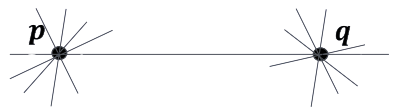
\includegraphics[width=0.25\linewidth]{images/deg2.png}
            \end{figure}
        \item When $\textnormal{rank}(C^{*}) = 1$, any symmetric $3 \times 3$ matrix $C^{*}$ can be expressed as:
            \[C^{*}=pp^T\]
            In this situation, the conic corresponds to the line $l$ going through point $p$ repeated twice. 
            \begin{figure}[H]
                \centering
                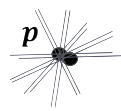
\includegraphics[width=0.1\linewidth]{images/deg1.png}
            \end{figure}
    \end{itemize}

    \begin{definition}
        The degenerate dual conic $C^{*}=pq^T+qp^T$ going through two circular point $p$ and $q$ is known as the \emph{conic dual to the circular points}, and it can be expressed as:
        \[C^{*}_{\infty}=IJ^{T}+JI^{T}=
        \begin{bmatrix}
            1 & 0 & 0 \\
            0 & 1 & 0 \\
            0 & 0 & 0 
        \end{bmatrix}\]
    \end{definition}

\newpage

\section{Transformations}
    \begin{definition}
        A \emph{projective mapping} between a projective plane $\mathbb{P}^2$ and another projective plane $\mathbb{P}^{'2}$ is an invertible mapping which preserves co-linearity:
        \[h:\mathbb{P}^2 \rightarrow \mathbb{P}^{'2}, x^{'}=h(x),x_1,x_2,x_3 \textnormal{ are colinear}\]
        \[\Leftrightarrow\]
        \[x_1^{'}=h(x_1),x_2^{'}=h(x_2),x_3^{'}=h(x_3) \textnormal{ are colinear}\]
    \end{definition}
    Projective mapping is also called projectivity or homography. 
    \begin{example}
        Mappings between two planes induced by central projection are projective, since they preserve co-linearity. 
        \begin{figure}[H]
            \centering
            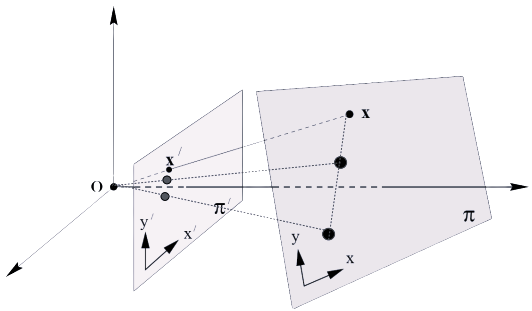
\includegraphics[width=0.4\linewidth]{images/map1.png}
        \end{figure}
        Mapping between a planar scene and its image is a homography, since it is induced by a central projection
        \begin{figure}[H]
            \centering
            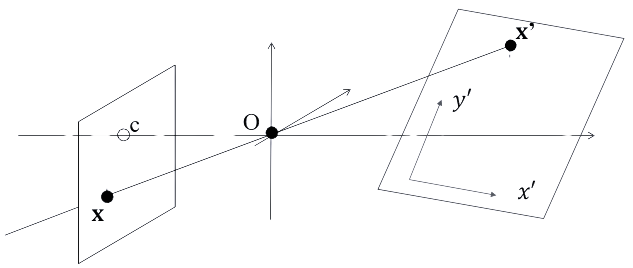
\includegraphics[width=0.4\linewidth]{images/map2.png}
        \end{figure}
        Mapping between two images of a planar scene is a homography.
        \begin{figure}[H]
            \centering
            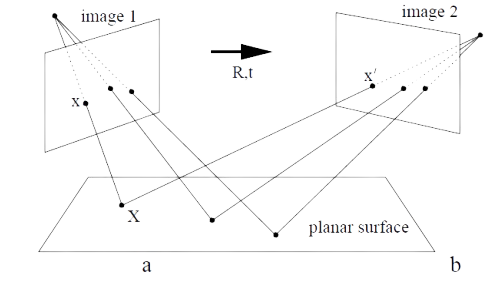
\includegraphics[width=0.4\linewidth]{images/map3.png}
        \end{figure}
        Two images of a 3D scene, taken by a camera rotating around its center are related by a homography, since the second image is a central projection of the first image. 
        \begin{figure}[H]
            \centering
            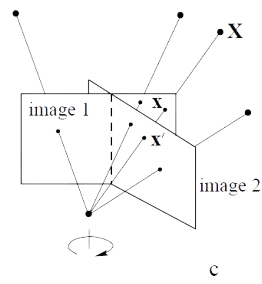
\includegraphics[width=0.3\linewidth]{images/map4.png}
        \end{figure}
        The shadow cast by a planar silhouette onto a ground plane is a projective transformation of the planar silhouette, since they are related by a central projection. 
        \begin{figure}[H]
            \centering
            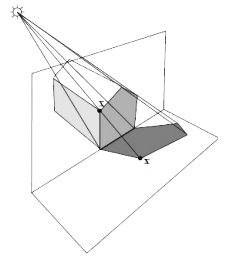
\includegraphics[width=0.3\linewidth]{images/map5.png}
        \end{figure}
    \end{example}
    \begin{theorem}
        A mapping $h:\mathbb{P}^{2} \rightarrow \mathbb{P}^{'2}$ is projective if and only if there exists an invertible $3 \times 3$ matrix $H$ such that for any point in $\mathbb{P}^{2}$ represented by the vector $x$, is $h(x)=Hx$, where: 
        \[H=\begin{bmatrix}
            h_{11} & h_{12} & h{13} \\
            h_{21} & h_{22} & h{23} \\
            h_{31} & h_{32} & h{33} 
        \end{bmatrix}\]
    \end{theorem}
    Projective mappings are linear when expressed in homogeneous coordinates, but they do not exhibit linearity when represented in Cartesian coordinates.

    According to the theorem, if we have $h(x)=x^{'}=Hx$, then multiplying the matrix $H$ by any nonzero scalar $\lambda$ still satisfies the relation for the same points, giving us $x^{'}=\lambda Hx$. 
    Therefore, any nonzero scalar multiple of the matrix $H$ represents the same projective mapping as $H$.
    As a result, we can conclude that $H$ is a homogeneous matrix.
    Despite having nine entries, it possesses only eight degrees of freedom, specifically the ratios between its elements. 
    Consequently, we can estimate $H$ using just four point correspondences.
    Each point correspondence, expressed as $x^{'}=Hx$, provides two independent equations in this estimation process.
    \newpage
    \begin{definition}
        A \emph{homography} transforms various geometric entities as follows:
        \begin{enumerate}
            \item It maps a point $x$ to a point $x^{'}$, where the transformation is expressed as: 
                \[x \rightarrow H x=x^{'}\]
            \item It maps a line $l$ to a line $l^{'}$, and this transformation is represented as: 
                \[l \rightarrow H^{-T} l=l^{'}\]
            \item It maps a conic $C$ to a conic $C^{'}$, and the transformation is given by: 
                \[C \rightarrow H^{-T} CH^{-1}=C^{'}\]
            \item It maps a dual conic $C^{*}$ to a dual conic $C^{*'}$, with the transformation being: 
                \[C^{*} \rightarrow H C^{*}H^{T}=C^{*'}\]
        \end{enumerate}
    \end{definition}
    \begin{proof}[of mapping two]
        To transform the equation of the line in terms of $x$, given by $l^Tx=0$, into a constraint on $x^{'}=Hx$, we combine the two equations, resulting in a linear equation on $x^{'}$: 
        \[l^{'T}x^{'}=0\]
        Here, $l^{'T}=l^{T}H^{-1}$. 
        Thus, we have:
        \[l^{'}=H^{-T}l\]
    \end{proof}
    \begin{proof}[of mapping three]
        To transform the equation of the conic in terms of $x$, given by $x^{T}Cx=0$, into a constraint on $x^{'}=Hx$, we have$x=H^{-1}x^{'}$ and $x^{T}=x^{iT}H^{-T}$. 
        Combining these three equations, we obtain a linear equation on $x^{'}$: 
        \[x^{'T}C^{'}x^{'}=0\]
        Hence, we have:
        \[C^{'}=H^{-T} CH^{-1}\]
    \end{proof}
    \begin{proof}[of mapping four]
        or the transformation of a dual conic, we apply the same idea, yielding:
        \[C^{*'}=H C^{*}H^{T}\]
    \end{proof}
    The point-line incidence is preserved. 
    \begin{proof}
        Let $x$ be a point on the line $l$. 
        This is expressed as $l^Tx=0$. 
        When we apply the projective transformation $H$ to both $x$and $l$, resulting in $Hx=x^{'}$ and $H^{-1}l=l^{'}$, they remain incident if $l^{'T}x^{'}=0$:
        \[l^{'T}x^{'}=l^{T}H^{-1}x^{'}=l^{T}H^{-1}Hx=l^{T}x=0\]
    \end{proof}

    \subsection{Vanishing points and vanishing line}
    The point that is common to both parallel lines $l_1={\begin{bmatrix} a & b & c_1 \end{bmatrix}}^{T}$ and $l_2={\begin{bmatrix} a & b & c_2 \end{bmatrix}}^{T}$ is the point $x={\begin{bmatrix} b & -a & 0 \end{bmatrix}}^{T}$. 
    This point is situated at infinity along the direction of both lines.
    When seeking the common point of the infinite lines $l_i$, we find that they all share the same point:
    \[x_{\infty}={\begin{bmatrix} b & -a & 0 \end{bmatrix}}^{T}\]
    Hence, it becomes apparent that all these lines converge at ${\begin{bmatrix} b & -a & 0 \end{bmatrix}}^{T}$. 
    
    If we apply a projective transformation to all the aforementioned parallel lines $l_i$, we obtain the transformed lines $l_i^{'}$. 
    The common point $x_{\infty}$, shared by all lines $l_i$, is mapped to a point $x_{\infty}^{'}$ which belongs to each of the lines $l_i^{'}$. 
    \begin{figure}[H]
        \centering
        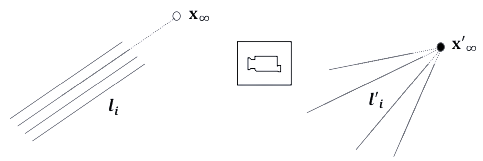
\includegraphics[width=0.5\linewidth]{images/vanishing.png}
    \end{figure}
    Therefore, we can assert that all lines $l_i^{'}$ intersect at the point $x_{\infty}^{'}=Hx_{\infty}$, referred to as the vanishing point associated with the direction $(b,-a)$ of the parallel lines. 
    \begin{theorem}
        The image of a set of parallel lines $l_i$ is a set of lines $l_i^{'}$ concurrent at a common point $x^{'}$ known as the vanishing point of the direction of lines $l_i$. 
    \end{theorem}

    By applying a projective transformation to the line at infinity $l_{\infty}$, we obtain a line $l_{\infty}^{'}$. 
    This line intersects the image all the points at the infinity $x_{\infty}$ from  the original plane. 
    Consequently, the vanishing line $l_{\infty}^{'}$ can be determined from two vanishing points. 
    \begin{figure}[H]
        \centering
        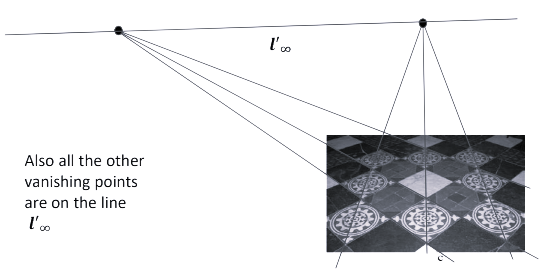
\includegraphics[width=0.5\linewidth]{images/vanishingline.png}
    \end{figure}

    \subsection{Polarity}
    Polarity remains unaltered in the presence of projective mappings.
    The polar line $l=Cx$ corresponding to a point $x$ with respect to a conic $C$ gets mapped to the polar line of the transformed point $x^{'} = Hx$ with respect to the transformed conic:
    \[C^{'}=H^{-T}CH^{-1}\]
    \begin{proof}
        This property holds because:
        \[C^{'}x^{'}=H^{-T}CH^{-1}Hx=H^{-T}Cx=H^{-T}l=l^{'}\]
        Therefore, the polar line of the transformed point aligns with the polar line of the original point.
    \end{proof}
    \begin{figure}[H]
        \centering
        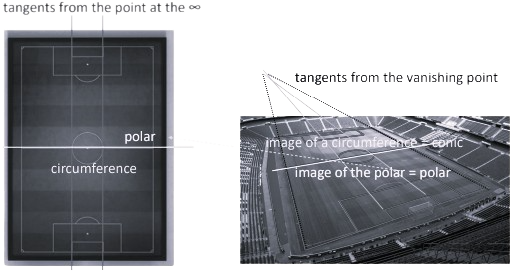
\includegraphics[width=0.75\linewidth]{images/polarity.png}
    \end{figure}
    In conclusion, as polarity remains intact under projective mappings, conjugacy is similarly preserved, and the relationship $CR=-1$ is also upheld.

    \subsection{Cross ratio}
    Given a line defined by four points with the following relationships:
    \[x_1=\propto_1Y+\beta_1Z\]
    \[x_2=\propto_2Y+\beta_2Z\]
    The cross ratio is expressed as:
    \[CR_{X_1,X_2,Y,Z}=\dfrac{\beta_1/\alpha_1}{\beta_2/\alpha_2}\]
    Upon applying a projective transformation $H$ to these four points:
    \[Y^{'}=HY \:\:\:\:\:\: Z^{'}=HZ\] 
    \[x^{'}_1=HX_1=x_1=\propto_1Y^{'}+\beta_1Z^{'} \:\:\:\:\:\: x^{'}_2=HX_2=\propto_2Y^{'}+\beta_2Z^{'}\]
    The coefficients of the linear combination remain the same. 
    Hence, the cross ratio is conserved, maintaining its original value:
    \[CR_{X_1^{'},X_2^{'},Y^{'},Z^{'}}=\dfrac{\beta_1/\alpha_1}{\beta_2/\alpha_2}=CR_{X_1,X_2,Y,Z}\]

    \subsection{Isometries}
    Isometries possess three degrees of freedom, which include translation denoted as $t$ and the rotation angle represented by $\vartheta$. 
    Consequently, the invariants of this transformation encompass lengths, distances, and areas.
    \begin{figure}[H]
        \centering
        
\includegraphics[width=0.25\linewidth]{images/isometry.png}
    \end{figure}
    \begin{definition}
        The \emph{orthogonal matrix} $R_{\perp}$ is defined as follows: 
        \[R_{\perp}^{-1}=R_{\perp}^{T}\]
    \end{definition}
    Hence, the matrix $H_I$ for isometries takes the following form:
    \[H_I=
    \begin{bmatrix}
        \cos \vartheta & -\sin \vartheta & t_x \\
        \sin \vartheta & \cos \vartheta & t_y \\
        0 & 0 & 1
    \end{bmatrix}\]
    Here, $
    \begin{bmatrix}
        \cos \vartheta & -\sin \vartheta \\
        \sin \vartheta & \cos \vartheta
    \end{bmatrix}
    =R_{\perp}$
    \begin{figure}[H]
        \centering
        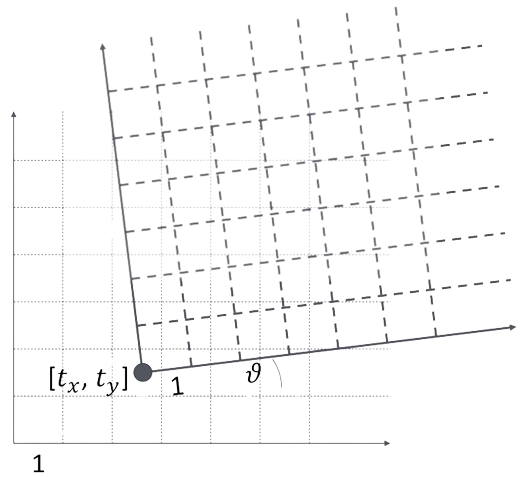
\includegraphics[width=0.25\linewidth]{images/isometry1.png}
        \caption{Isometry}
    \end{figure}

    \subsection{Similarities}
    Similarities are characterized by four degrees of freedom, encompassing the translation, denoted as $t$; the scale, represented by $s$; and the rotation angle, expressed as $\vartheta$.
    Consequently, the invariants of this transformation encompass the ratio of lengths and angles.
    Furthermore, the circular points $I$ and $J$ remain invariant throughout this transformation.
    \begin{figure}[H]
        \centering
        
\includegraphics[width=0.2\linewidth]{images/similarity.png}
    \end{figure}
    Hence, the matrix $H_S$ for similarities is as follows:
    \[H_I=
    \begin{bmatrix}
        s\cos \vartheta & -s\sin \vartheta & t_x \\
        s\sin \vartheta & s\cos \vartheta & t_y \\
        0 & 0 & 1
    \end{bmatrix}\]
    Here, $
    \begin{bmatrix}
        s\cos \vartheta & -s\sin \vartheta \\
        s\sin \vartheta & s\cos \vartheta
    \end{bmatrix}
    =sR_{\perp}$
    \begin{figure}[H]
        \centering
        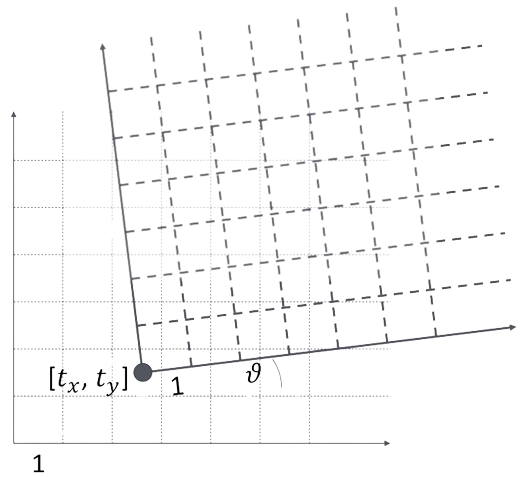
\includegraphics[width=0.25\linewidth]{images/isometry1.png}
        \caption{Similarity}
    \end{figure}

    \subsection{Affinities}
    Affinities exhibit six degrees of freedom, consisting of the sub-matrix $A$ and the translation component. 
    As a result, the invariants of this transformation encompass parallelism, the ratio of parallel lengths, and the ratio of areas. 
    The matrix $A$ is defined as a $2 \times 2$ matrix with a rank of two. 
    Additionally, the line at infinity, denoted as $l_{\infty}$, remains invariant throughout the transformation.
    \begin{figure}[H]
        \centering
        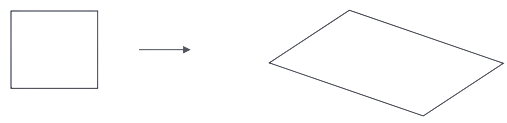
\includegraphics[width=0.25\linewidth]{images/affinities.png}
    \end{figure}
    Hence, the matrix $H_A$ for affinities takes the following form:
    \[H_I=
    \begin{bmatrix}
        a_{11} & a_{21} & t_x \\
        a_{12} & a_{21} & t_y \\
        0 & 0 & 1
    \end{bmatrix}\]
    Here, $
    \begin{bmatrix}
        a_{11} & a_{21} \\
        a_{12} & a_{21} \\
    \end{bmatrix}
    =A$
    \begin{figure}[H]
        \centering
        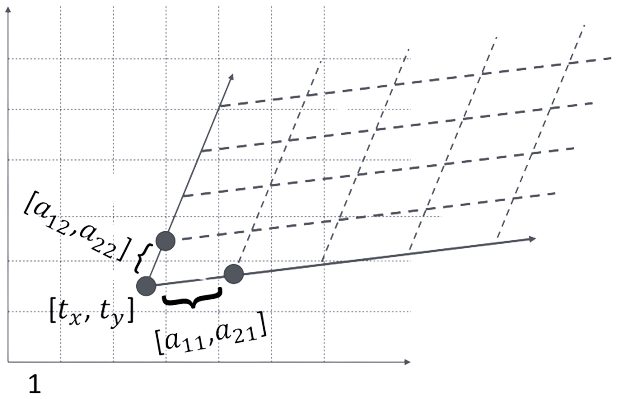
\includegraphics[width=0.3\linewidth]{images/affinities1.png}
    \end{figure}

    \subsection{Projectivities}
    Projectivities possess eight degrees of freedom, encompassing the sub-matrix $A$, the vector $v$, and the translation component. 
    Therefore, the invariants of this transformation include co-linearity, incidence, and the order of contact.
    The matrix $A$ is defined as a $2 \times 2$ matrix with a rank of two. 
    Furthermore, the cross ratio remains invariant throughout this transformation.
    \begin{figure}[H]
        \centering
        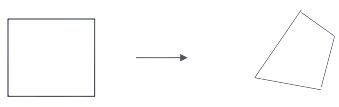
\includegraphics[width=0.25\linewidth]{images/projectivities.png}
    \end{figure}
    Hence, the matrix $H_P$ for projectivities takes the following form:
    \[H_I=
    \begin{bmatrix}
        a_{11} & a_{21} & t_x \\
        a_{12} & a_{21} & t_y \\
        v_1 & v_2 & 1
    \end{bmatrix}\]
    Here, $
    \begin{bmatrix}
        a_{11} & a_{21} \\
        a_{12} & a_{21} \\
    \end{bmatrix}
    =A$
    \begin{figure}[H]
        \centering
        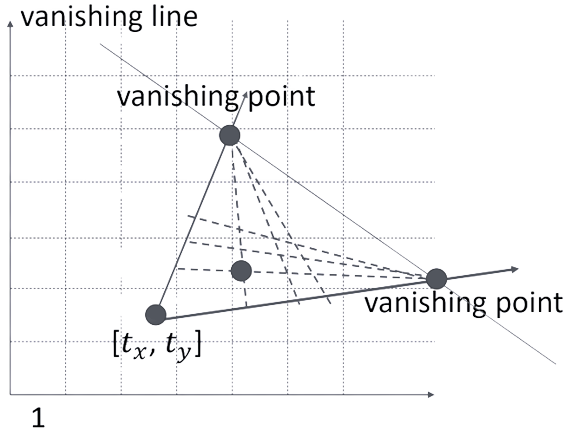
\includegraphics[width=0.25\linewidth]{images/projectivities1.png}
        \caption{Affinity}
    \end{figure}

\newpage

\chapter{Two-dimensional reconstruction}
    \section{Introduction}
    When we aim to recover a model of an unknown planar scene based on an image of the scene, which is a projective transformation denoted as $x_i^{'}=Hx_i$, we face a significant challenge.
    The key issue is that we know the values of $x_i$ (the scene points), but we don't have direct knowledge of the transformation matrix $H$, which complicates a straightforward inversion of the mapping.
    
    The general problem is inherently unsolvable due to the excessive number of unknown variables. 
    To tackle this challenge, we can adopt two primary strategies:
     
    \begin{enumerate}
        \item Reduce unknowns: in many cases, it is unnecessary to precisely recover the original scene configuration. 
            Instead, the objective is to retrieve the overall shape of the scene, known as shape reconstruction. 
            By doing so, we can reduce the number of unknowns from eight to four, and the matrix $H$ takes on the following form:
            \[H=    
            \begin{bmatrix}
                s\cos \vartheta & -s\sin \vartheta & t_x \\
                s\sin \vartheta & s\cos \vartheta & t_y \\
                0 & 0 & 1
            \end{bmatrix}\]
            Additionally, it's possible to perform similarity reconstruction, which reduces the unknowns by two, or affine reconstruction, which reduces the unknowns by six.
        \item Add constraints: this strategy involves utilizing extra information to recover a model of the scene. 
            The valuable information typically pertains to parameters that remain invariant under the desired class of mappings but are not invariant under more general classes.
    \end{enumerate}

    The reconstruction can fall into one of two categories:
    \begin{itemize}
        \item Affine reconstruction: in this scenario, the reconstructed scene is an affine mapping of the original scene.
        \item Shape reconstruction: in this case, the reconstructed scene follows a similarity mapping of the original scene, aiming to capture the overall shape while simplifying the problem.
    \end{itemize}

    \section{Affine reconstruction}
    \begin{theorem}
        A projective transformation $H$ that maps the line at the infinity $l_{\infty}$ onto itself implies that $H$ is affine. 
    \end{theorem}
    \begin{proof}
        A point at the infinity $x_{\infty}={\begin{bmatrix} x & y & 0 \end{bmatrix}^T}$ is mapped to another point $x^{'}=Hx_{\infty}$ that remains at infinity only if the third coordinate of $x'$ is zero.
        For all $(x,y)$, this condition is expressed as:
        \[\begin{bmatrix} v_1 & v_2 & 1 \end{bmatrix} \begin{bmatrix} x \\ y \\ 0 \end{bmatrix}=0 \rightarrow \begin{bmatrix} v_1 & v_2 & 1 \end{bmatrix} = \begin{bmatrix} 0 & 0 & 1 \end{bmatrix}\]
        In other words, $H$ is affine.
    \end{proof}
    The image provided results from a general projective mapping of the original scene. 
    Consequently, the vanishing line $l^{'}_{\infty}$ in the image differs from the original $l_{\infty}$. 
    This observation leads to the possibility of using $l^{'}_{\infty}$ as additional information.
    By applying a new projective transformation $H_{AR}$ to the image that restores $l^{'}_{\infty}$ to $l_{\infty}$, a modified image is obtained.
    Notably, the image of the line at infinity $l_{\infty}$ in this new model remains as $l_{\infty}$. 

    Based on the theorem, the resulting model (i.e., the new image) is an affine mapping of the original scene. 
    Therefore, the achieved model is an affine reconstruction of the scene.
    \begin{figure}[H]
        \centering
        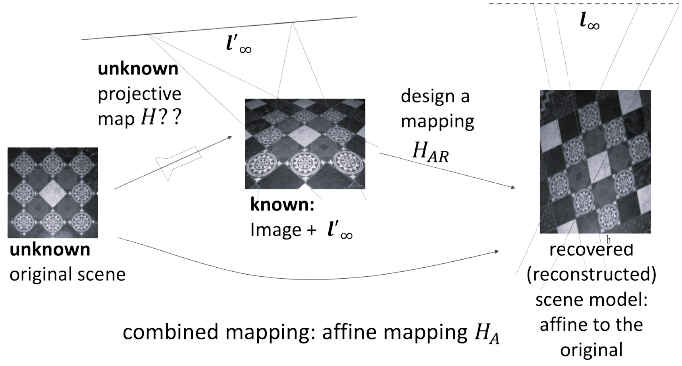
\includegraphics[width=0.75\linewidth]{images/HAR.png}
    \end{figure}
    The challenges associated with this approach include:
    \begin{itemize}
        \item Determine a projective transformation $H_{AR}$ that restores $l^{'}_{\infty}$ to $l_{\infty}$.
        \item Identify the vanishing line.
    \end{itemize}
    
    \subsection{Determine a projective transformation}
    To find a projective mapping $H_{AR}$ that restores $l^{'}_{\infty}$ to $l_{\infty}$ the mapping should satisfy the condition of mapping any point $x^{'} \in l^{'}_{\infty}$ onto a set of point at infinity: 
    \[H_{AR}x^{'} = \begin{bmatrix} * \\ * \\ 0 \end{bmatrix}\]
    The mapping can be effectively represented as:
    \[H_{AR}=
    \begin{bmatrix}
        * & * & * \\
        * & * & * \\
        \: & l^{'T}_{\infty} & \:
    \end{bmatrix}\]
    In this matrix representation, we achieve the desired mapping: 
    \[H_{AR}x^{'}=
    \begin{bmatrix}
        * & * & * \\
        * & * & * \\
        \: & l^{'T}_{\infty} & \:
    \end{bmatrix}
    x^{'}
    =
    \begin{bmatrix}
        * \\
        * \\
        l^{'T}_{\infty}x^{'}
    \end{bmatrix}
    \]

    \subsection{Identify the vanishing line}
    To determine the vanishing line, additional information can be employed, such as the image of parallel lines.
    \begin{figure}[H]
        \centering
        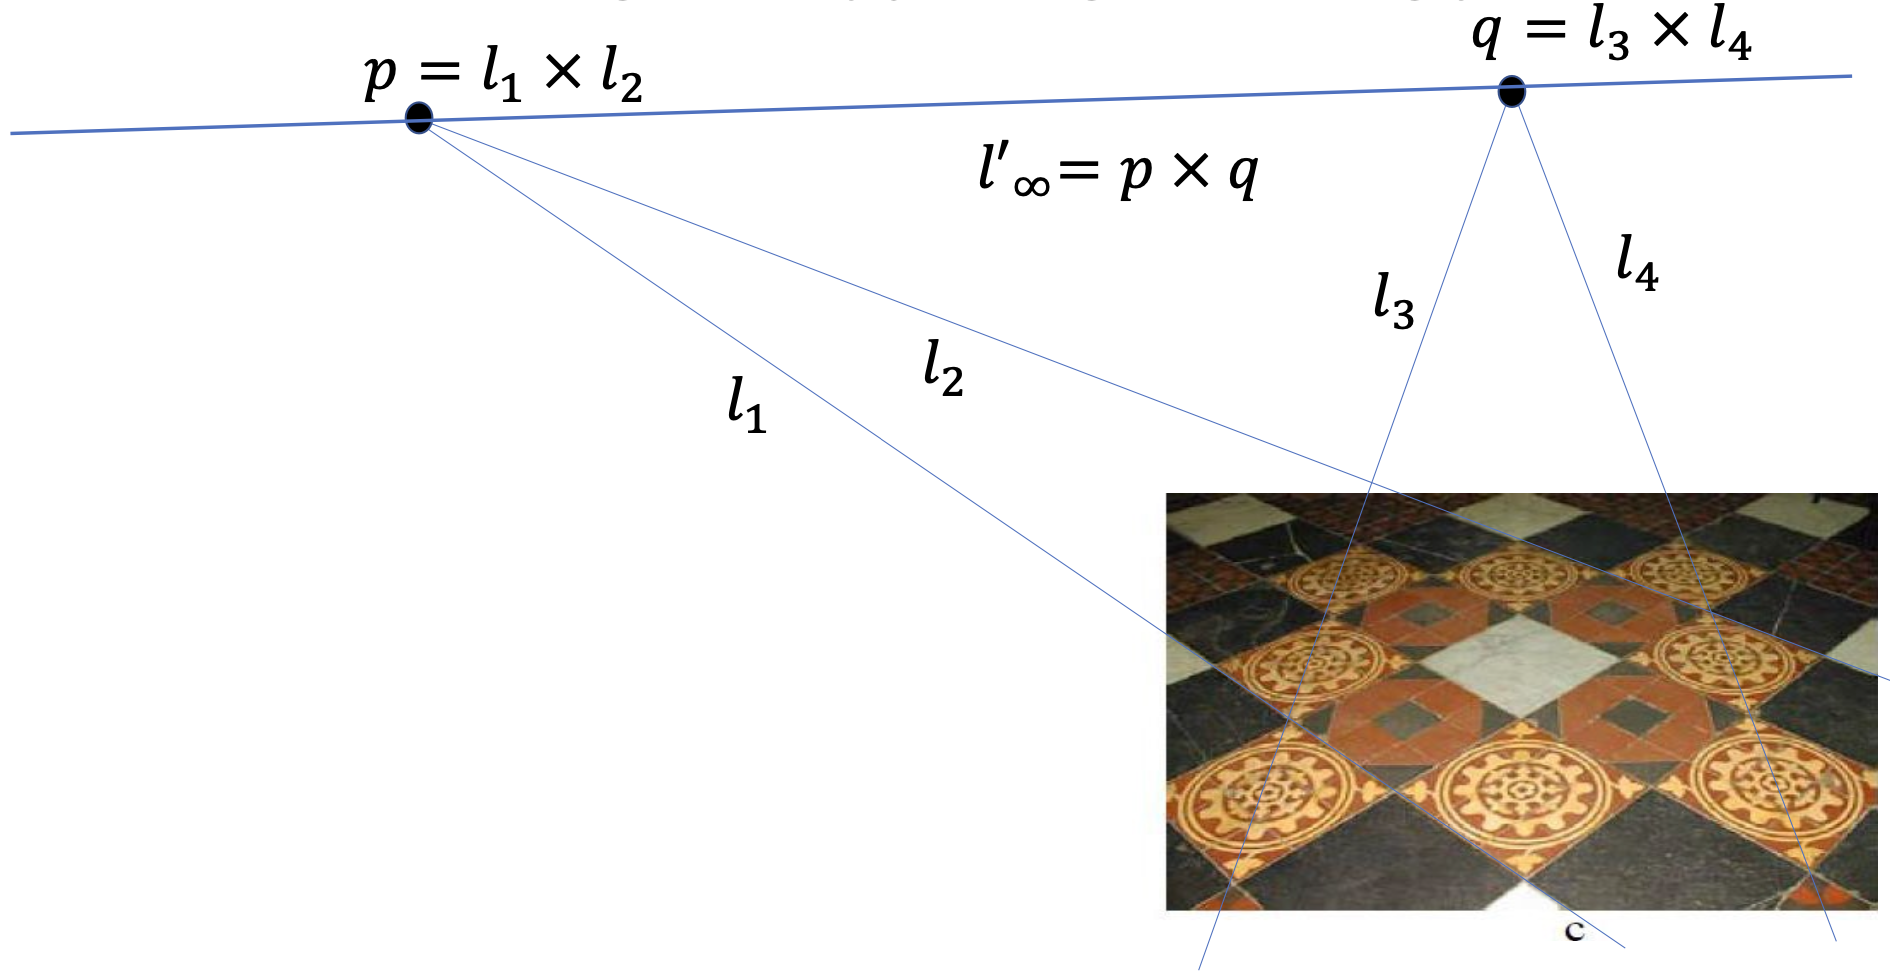
\includegraphics[width=0.5\linewidth]{images/van.png}
    \end{figure}

    \section{Shape reconstruction}
    \begin{theorem}
        A projective transformation $H$ that maps the circular points $I$ and $J$ onto themselves implies that $H$ is a similarity transformation. 
    \end{theorem}
    \begin{proof}
        When we multiply a similarity matrix $H_S$ by the circular point $I$, we obtain a multiple of $I$.
        Similarly, the same result is obtained for the other circular point, $J$.
    \end{proof}
    The given image represents a general projective mapping of the original scene. 
    Consequently, the image of the circular points, denoted as $(I^{'},J^{'})$, differs from $I$ and $J$. 
    To utilize $I^{'},J^{'}$ as additional information, we apply a new projective mapping $H_{SR}$ to map $I^{'},J^{'}$ back to $I,J$. 
    This process generates a new modified image where the circular points $I,J$ are restored.
    As per the theorem, the obtained model (new image) is similar to the original scene, representing a shape reconstruction of the scene.
    \begin{figure}[H]
        \centering
        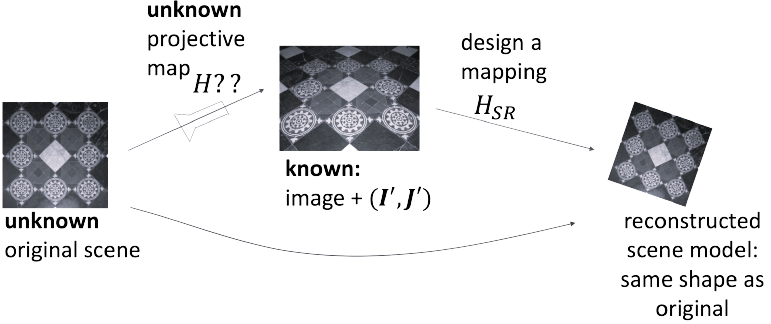
\includegraphics[width=0.75\linewidth]{images/HSR.png}
    \end{figure}
    The method comes with certain challenges:
    \begin{itemize}
        \item Finding a projective mapping $H_{SR}$ that restores $I^{'},J^{'}$ to $I,J$. 
        \item Determining the vanishing line.
    \end{itemize}
    
    \subsection{Identify a projective transformation}
    Discovering a projective transformation $H_{SR}$ that restores $I^{'}, J^{'}$ to $I, J$ is equivalent to finding one of the $\infty^{4}$ matrices that satisfy:
    \[\begin{cases}
        H_{SR}I^{'}=I \\
        H_{SR}J^{'}=J
    \end{cases}\]
    This task can be quite challenging.
    
    Let's utilize alternative information: the degenerate conic dual to $I^{'},J^{'}$, represented as $C_{\infty}^{'*}=I^{'}J^{'T}+J^{'}I^{'T}$, which corresponds to the image of the original conic dual to the circular points $(I,J)$, expressed as: 
    \[C_{\infty}^{*}=IJ^{T}+JI^{T}\]
    Since $(I^{'},J^{'})$ is the image of $(I,J)$, then also $C_{\infty}^{'*}$ is the image of $C_{\infty}^{*}$. 
    As a result, any projective transformation $H_{SR}$ that restores $(I^{'},J^{'})$ to $(I,J)$ also restores $C_{\infty}^{'*}$ to $C_{\infty}^{*}$. 
    By applying the transformation rule for dual conics under projective mappings, we get:
    \[C^{*}_{\infty}=H_{SR}C^{'*}_{\infty}H_{SR}^T\]
    Reversing this relationship, we find:
    \[C_{\infty}^{'*}=H_{SR}^{-1} 
    \begin{bmatrix}
        1 & 0 & 0 \\
        0 & 1 & 0 \\
        0 & 0 & 0
    \end{bmatrix}
    H_{SR}^{-T}\]
    Applying singular value decomposition (SVD) to this equation, we find that the matrices $H_{SR}^{-1}$ and $H_{SR}^{-T}$ are orthogonal. 
    Consequently, we have:
    \[\textnormal{SVD}(C_{\infty}^{'*})=U_\perp
    \begin{bmatrix}
        1 & 0 & 0 \\
        0 & 1 & 0 \\
        0 & 0 & 0
    \end{bmatrix}
    U_{\perp}^T\]
    Which provides a unique solution: $H_{SR}=U_{\perp}^{-1}=U_{\perp}^T$. 
    To address the issues with image rectification, we need to modify the matrix $H_{SR}$ as follows:
    \[H_{SR}=
    \begin{bmatrix}
        \frac{1}{\sqrt{a}} & 0 & 0 \\
        0 & \frac{1}{\sqrt{b}} & 0 \\
        0 & 0 & 1
    \end{bmatrix}
    U^T
    \]

    \subsection{Determine the vanishing line}
    To determine the vanishing line, one can leverage additional information from the observed scene. 
    This information can be used to establish the following constraints:
    \begin{enumerate}
        \item Known angles between lines: when the angles between lines in the scene are known, these angles can be used to constrain the vanishing line. 
            The angle between two lines is related to the angle between their normal directions and is independent of parameters $c_1$ and $c_2$. 
            Mathematically, this relationship is expressed as:
            \[\cos\vartheta=\dfrac{a_1a_2+b_1b_2}{\sqrt{(a_1^2+b_1^2)(a_2^2+b_2^2)}}\]
            Here, $a_1$, $b_1$, $a_2$, and $b_2$ are coefficients of the normal vectors of the lines. 
            By rewriting the terms, this equation can be expressed as: 
            \[\cos\vartheta=\dfrac{l^TC_{\infty}^{*}m}{\sqrt{(l^TC_{\infty}^{*}l)(m^TC_{\infty}^{*}m)}}\]
            This equation can be further simplified by using the rules obtaining $C_{\infty}^{*}=H^{-1}C_{\infty}^{*'}H^{-T}$.  
            Now, we can rewrite $l^TC_{\infty}^{*}m$ as $l^{'T}C_{\infty}^{*'}m^{'}$. 
            With these transformations, the equation becomes:
            \[\cos\vartheta=\dfrac{l^{'T}C_{\infty}^{*'}m^{'}}{(l^{'T}C_{\infty}^{*'}l^{'})(m^{'T}C_{\infty}^{*'}m^{'})}\]
            In this case, $m^{'}$ and $l^{'}$ are obtained from the image. 
            Since the angle is known, this equation provides a linear constraint on $C_{\infty}^{*'}$, that is linear when the lines are perpendicular ($\cos\vartheta=0$).
            The unknown matrix $C_{\infty}^{'}$ is symmetric, homogeneous, and singular, providing four independent constraints.
        \item Known shape of objects: if the shape of objects in the scene is known, the reconstruction matrix $H_{SR}$ can be determined. 
            The transformation matrix is defined as:
            \[H_{SR}=
            \begin{bmatrix}
                \frac{1}{\sqrt{a}} & 0 & 0 \\
                0 & \frac{1}{\sqrt{b}} & 0 \\
                0 & 0 & 1
            \end{bmatrix}
            U^T
            \]
            The Euclidean reconstructed image is calculated as $M_S=H_{SR} \cdot \textnormal{image}$
        \item Combinations of constraints: it is also possible to use a combination of known angles between lines and the shape of objects for additional constraints.
        \item Observation of rigid planar motion: when observing rigid planar motion, which is a similarity transformation, the circular points remain invariant.
            The object has three degrees of freedom, and the center of rotation and the rotation angle can be determined.
            Given a matrix $H$, the eigenvectors of $H$ correspond to fixed points, and the eigenvectors of $H^{-T}$ correspond to fixed lines of the transformation.
            The eigenvectors can be used to extract important information:
            \begin{itemize}
                \item Eigenvectors $I^{'},J^{'}$ correspond to complex eigenvalues. 
                \item The phase of these eigenvectors is the rotation angle.
                \item Eigenvector $O^{'}$ correspond to real eigenvalues. 
            \end{itemize}
            The three eigenvectors of $H$ are proportional to three distinct values: 1, $e^{i\theta}$, and $-e^{i\theta}$.
            The eigenvector corresponding to the eigenvalue 1 represents the image of the center of rotation, denoted as $O$, and the angle $\theta$ corresponds to the rotation angle. 
            The eigenvectors associated with the complex eigenvalues represent the images of the circular points $I^{'},J^{'}$. 
            Therefore, using the relationship $C_{\infty}^{'*}=I^{'}J^{'T}+J^{'}I^{'T}$, the singular value decomposition can be applied to obtain $\textnormal{SVD}(C_{\infty}^{'*})=UC_{\infty}^{*}U^T$, where $U^T$ is the rectification matrix. 
            Two methods can be used to address this:
            \begin{itemize}
                \item Direct method: 
                    \begin{enumerate}
                        \item Find $C_{\infty}^{*'}$. 
                        \item Compute $H_{rect}$ for rectification. 
                    \end{enumerate}
                \item Stratified method: 
                    \begin{enumerate}
                        \item Perform affine reconstruction from projective to affine.
                        \item Perform shape reconstruction from affine to metric.
                    \end{enumerate}
            \end{itemize}
            In some cases, the stratified method reduces numerical errors, providing a more accurate result.
    \end{enumerate}

    \section{Accuracy issues}
    There are various accuracy issues when doing image rectification: 
    \begin{enumerate}
        \item Noise and numerical errors: noise and numerical errors in the input data can affect the accuracy of the rectification process. 
            It's essential to preprocess and filter the data to minimize these issues.
        \item Little information: when choosing lines to identify vanishing points, it's crucial to select lines that are sufficiently far apart. 
            Choosing lines that are too close to each other can lead to inaccuracies in vanishing point estimation and rectification.
        \item Vanishing point near infinity: in cases where the vanishing point is nearly at infinity, it can be challenging to perform accurate affine rectification. 
            To address this issue:
            \begin{itemize}
                \item Draw two lines in the scene that are perpendicular to the given lines in the image.
                    If the two new lines are not parallel, adjust one of the intersection points to make them parallel.
                    \begin{figure}[H]
                        \centering
                        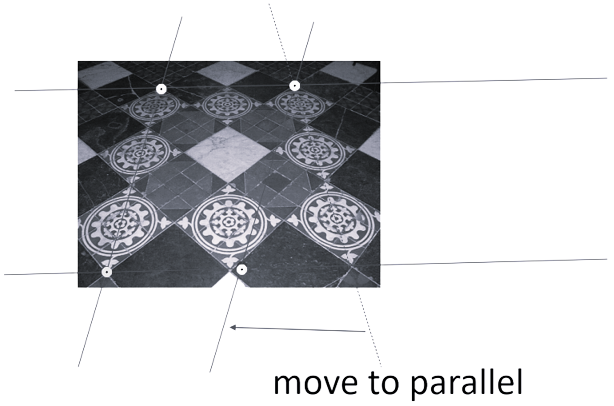
\includegraphics[width=0.4\linewidth]{images/vpi.png}
                    \end{figure}
                    Finally, apply affine reconstruction to obtain accurate results. 
                    \begin{figure}[H]
                        \centering
                        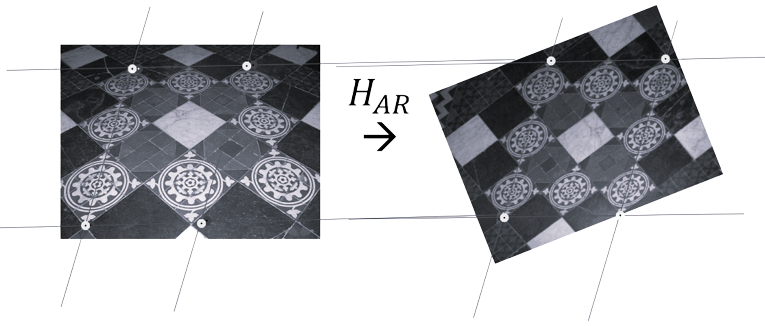
\includegraphics[width=0.5\linewidth]{images/ar.png}
                    \end{figure}
                \item When dealing with sets of parallel lines, you can choose one line from each set and randomly select another pair of lines, making sure they are perpendicular. 
                    With these four lines, you can compute the matrix product of $K$ and its transpose, denoted as $KK^T$, and then derive $K$ through Cholesky factorization.
                    Afterward, you can apply the rectifying transformation using the matrix:
                    \[H_{rect}=\begin{bmatrix}
                        K & t \\ 
                        0 & 1
                    \end{bmatrix}^{-1}\] 
            \end{itemize}
    \end{enumerate}
    The accuracy of image rectification is crucial for various computer vision and image processing applications, and addressing these issues is essential for obtaining reliable results.

\newpage

\chapter{Three-dimensional space projective geometry}
    \section{Introduction}
    In space geometry, the fundamental elements required for defining the geometry include points, planes, quadrics, and dual quadrics. 
    The allowable transformations within this type of geometry encompass projectivities, affinities, similarities, and isometries.

    \section{Points}
    Points in space geometry can be represented in Cartesian coordinates by defining a Euclidean space with its origin. 
    This approach allows for the unambiguous definition of every point using three Cartesian coordinates $(x, y, z)$.

    However, when analyzing images, it is more convenient to employ homogeneous coordinates. 
    The relationship between Cartesian and homogeneous coordinates is as follows:    \[
    X =
    \begin{bmatrix}
        x \\
        y \\
        z \\
        w
    \end{bmatrix}
    =w
    \begin{bmatrix}
        X \\
        Y \\
        Z \\
        1 
    \end{bmatrix}
    \]
    This representation exhibits homogeneity, meaning any vector $x$ is equivalent to all its non-zero multiples $\lambda x$, where $\lambda \neq 0$, since they all represent the same point.
    The null vector, however, does not represent any point.
    \begin{definition}
        The \emph{projective space} is defined as:
        \[\mathbb{P}^3=\{{\begin{bmatrix} x & y & z & w \end{bmatrix}}^T \in \mathbb{R}^4\}-\{{\begin{bmatrix} 0 & 0 & 0 & 0 \end{bmatrix}}^T\}\]
    \end{definition}

    \section{Planes}
    In the homogeneous coordinates, planes are defined by using the matrix: 
    \[\pi=\begin{bmatrix} a \\ b \\c \\d \end{bmatrix}\]
    Here, the direction normal to the plane is given by $(a, b, c)$, and the distance from the origin to the plane is calculated as:
    \[\textnormal{distance}=-\dfrac{d}{\sqrt{a^2+b^2+c^2}}\]
    Similar to homogeneous point coordinates, this representation of planes also exhibits the homogeneity property.
    Any vector $\pi$ is equivalent to all its non-zero multiples $\lambda \pi$, where $\lambda \neq 0$, as they all represent the same plane.
    The parameters $a, b, c, d$ are referred to as the homogeneous parameters of the plane.
    As with points, there are an infinite number of equivalent representations for a single plane, which includes all non-zero multiples of the unit normal vector.
    The null vector does not represent any plane. 
    If $d=0$, it signifies that the plane $\pi$ passes through the origin of space.

    To determine whether a point lies on a plane or if a plane passes through a point, you can solve the following system of equations:
    \[
    \begin{cases}
        ax+by+cz+dw=0 \\
        \pi^TX=X^T\pi=0
    \end{cases}
    \]
    \begin{definition}
        The plane 
        \[\begin{bmatrix} 0 & 0 & 0 & 1 \end{bmatrix} \begin{bmatrix} x \\ y \\ z \\ w \end{bmatrix}=w=0\] 
        is called the \emph{plane at the infinity} $\pi_{\infty}={\begin{bmatrix} 0 & 0 & 0 & 1 \end{bmatrix}}^T$. 
    \end{definition}
    It's important to note that this plane has an undefined normal direction.

\end{document}